% Appendices

%========================================
% APPENDIX 1: ADDITIONAL MATERIAL
%========================================
\chapter{Listings, Tabels and Figures}

\begin{lstlisting}[language=Python, caption=Preprocessing Function for images, label=PreprocessingFunction]
	def load_and_detect_faces(folder_path):
	images = []
	labels = []
	for label in os.listdir(folder_path):
	label_path = os.path.join(folder_path, label)
	if os.path.isdir(label_path):
	for img_file in os.listdir(label_path):
	img_path = os.path.join(label_path, img_file)
	img = cv2.imread(img_path, cv2.IMREAD_GRAYSCALE)
	if img is not None:
	# Detect face
	faces = face_cascade.detectMultiScale(img, scaleFactor=1.1, minNeighbors=5, minSize=(30, 30))
	for (x, y, w, h) in faces:
	# Crop to face region
	face_region = img[y:y+h, x:x+w]
	images.append(face_region)
	labels.append(label)
	images.append(cv2.flip(face_region, 1))
	labels.append(label)
	if label != "happy" or label != "neutral":
	images.append(imutils.rotate(face_region, 12))
	labels.append(label)
	if label == "fear":
	images.append(cv2.flip(imutils.rotate(face_region, 12), 1))
	labels.append(label)
	images.append(cv2.flip(imutils.rotate(face_region, 20), 1))
	labels.append(label)
	return images, labels
\end{lstlisting}

\begin{lstlisting}[language=Python, caption=Feature extraction functions for LBP and HOG, label=LBP_HOG]
	radius = 1
	n_points = 8 * radius
	
	def extract_lbp_features(images):
		lbp_features = []
		for img in images:
		
			img = cv2.resize(img, (64, 64))
			lbp = local_binary_pattern(img, n_points, radius, method='uniform')
			
			(hist, _) = np.histogram(lbp.ravel(), bins=np.arange(0, n_points + 3), range=(0, n_points + 2))
			
			hist = hist.astype("float")
			hist /= (hist.sum() + 1e-6)
			lbp_features.append(hist)
		return np.array(lbp_features)
	
	def extract_hog_features(images):
		hog_features = []
		
		pixels_per_cell = (10, 10)
		cells_per_block = (2,2)
		orientations = 9
		
		for img in images:
		
			img = cv2.resize(img, (80, 80))
			
			features = hog(
				img,
				orientations=orientations,
				pixels_per_cell=pixels_per_cell,
				cells_per_block=cells_per_block,
				block_norm='L2-Hys',
				transform_sqrt=True,
				feature_vector=True
			)
			hog_features.append(features)
		
		return np.array(hog_features)
\end{lstlisting}

\begin{lstlisting}[language=Python, caption=SVM - Model setup and training, label=SVM_Training]
	# Tests with GridSearchCV - abandoned because of overfitting on the training data
	# svm_rbf_pipe = make_pipeline(
	#     StandardScaler(),
	#     PCA(random_state=42),
	#     OneVsRestClassifier(SVC(kernel='rbf', gamma='scale', random_state=42))
	# )
	#
	# param_grid = {
		#     'n_components': [10, 20, 50, 40, 60, 80, 100, 200],
		#     'C': [0.1, 0.25, 1, 10, 100],
		#     'gamma': ['scale', 0.001, 0.01, 0.1]
		# }
	#
	# grid_search = GridSearchCV(
	#     estimator=svm_rbf_pipe,
	#     param_grid=param_grid,
	#     scoring='accuracy',
	#     cv=5,
	#     n_jobs=-1,
	#     verbose=2
	# )
	#
	# grid_search.fit(x_train, y_train)
	#
	# print(f"Best Parameters Found: {grid_search.best_params_}")
	# print(f"Best CV Score: {grid_search.best_score_:.4f}")
	#
	# best_model = grid_search.best_estimator_
	# y_train_pred = best_model.predict(x_train)
	# y_test_pred = best_model.predict(x_test)
	
	n_components = 1
	
	svm_rbf = make_pipeline(
	StandardScaler(),
	PCA(n_components=40),
	OneVsRestClassifier(SVC(kernel='rbf', C=0.45, gamma='scale'))
	)
	svm_rbf.fit(x_train, y_train)
	
	y_train_pred = svm_rbf.predict(x_train)
	y_test_pred = svm_rbf.predict(x_test)
\end{lstlisting}

\begin{longtable}[h]{c||c|c|c|c|c|c}  %[!h] steht für here, damit Tabelle an dieser Stelle eingefügt wird, ! für erzwungen
	& \textbf{Accuracy} & \textbf{MCC} & \textbf{F1} & \textbf{Accuracy} & \textbf{MCC} & \textbf{F1} \\
	& \textbf{Train} & \textbf{Train} & \textbf{Train} & \textbf{Test} & \textbf{Test} & \textbf{Test} \\ %\textbf macht die Elemente fettgeschrieben
	\hline
	\hline
	\textbf{KNN} & 65.8\% & 59.5\% & 64.8\% & 59.3\% & 51.7\% & 58.5\% \\
	\hline
	\textbf{SVM} & 82.1\% & 78.3\% & 81.8\% & 73.8\% & 68.3\% & 73.0\% \\
	\hline
	\textbf{DT} & 51.6\% & 46.3\% & 48.8\% & 46.7\% & 39.3\% & 43.8\% \\
	\hline
	\textbf{RF} & 58.6\% & 52.5\% & 52.0\% & 57.0\% & 50.6\% & 52.1\% \\
	\hline
	\textbf{Stack (KNN+DT+RF)} & 69.4\% & 63.3\% & 68.7\% & 61.0\% & 53.6\% & 60.0\% \\
	\hline
	\caption{Performance Results}
	\label{tbl:testing}
\end{longtable} 

\begin{figure}[h]
	\centering
	\includegraphics[width=1\textwidth]{figures/Emotions.png}
	\caption{Display of Emotions}
	\label{fig:emotions}
\end{figure}

\begin{figure}[h]
	\centering
	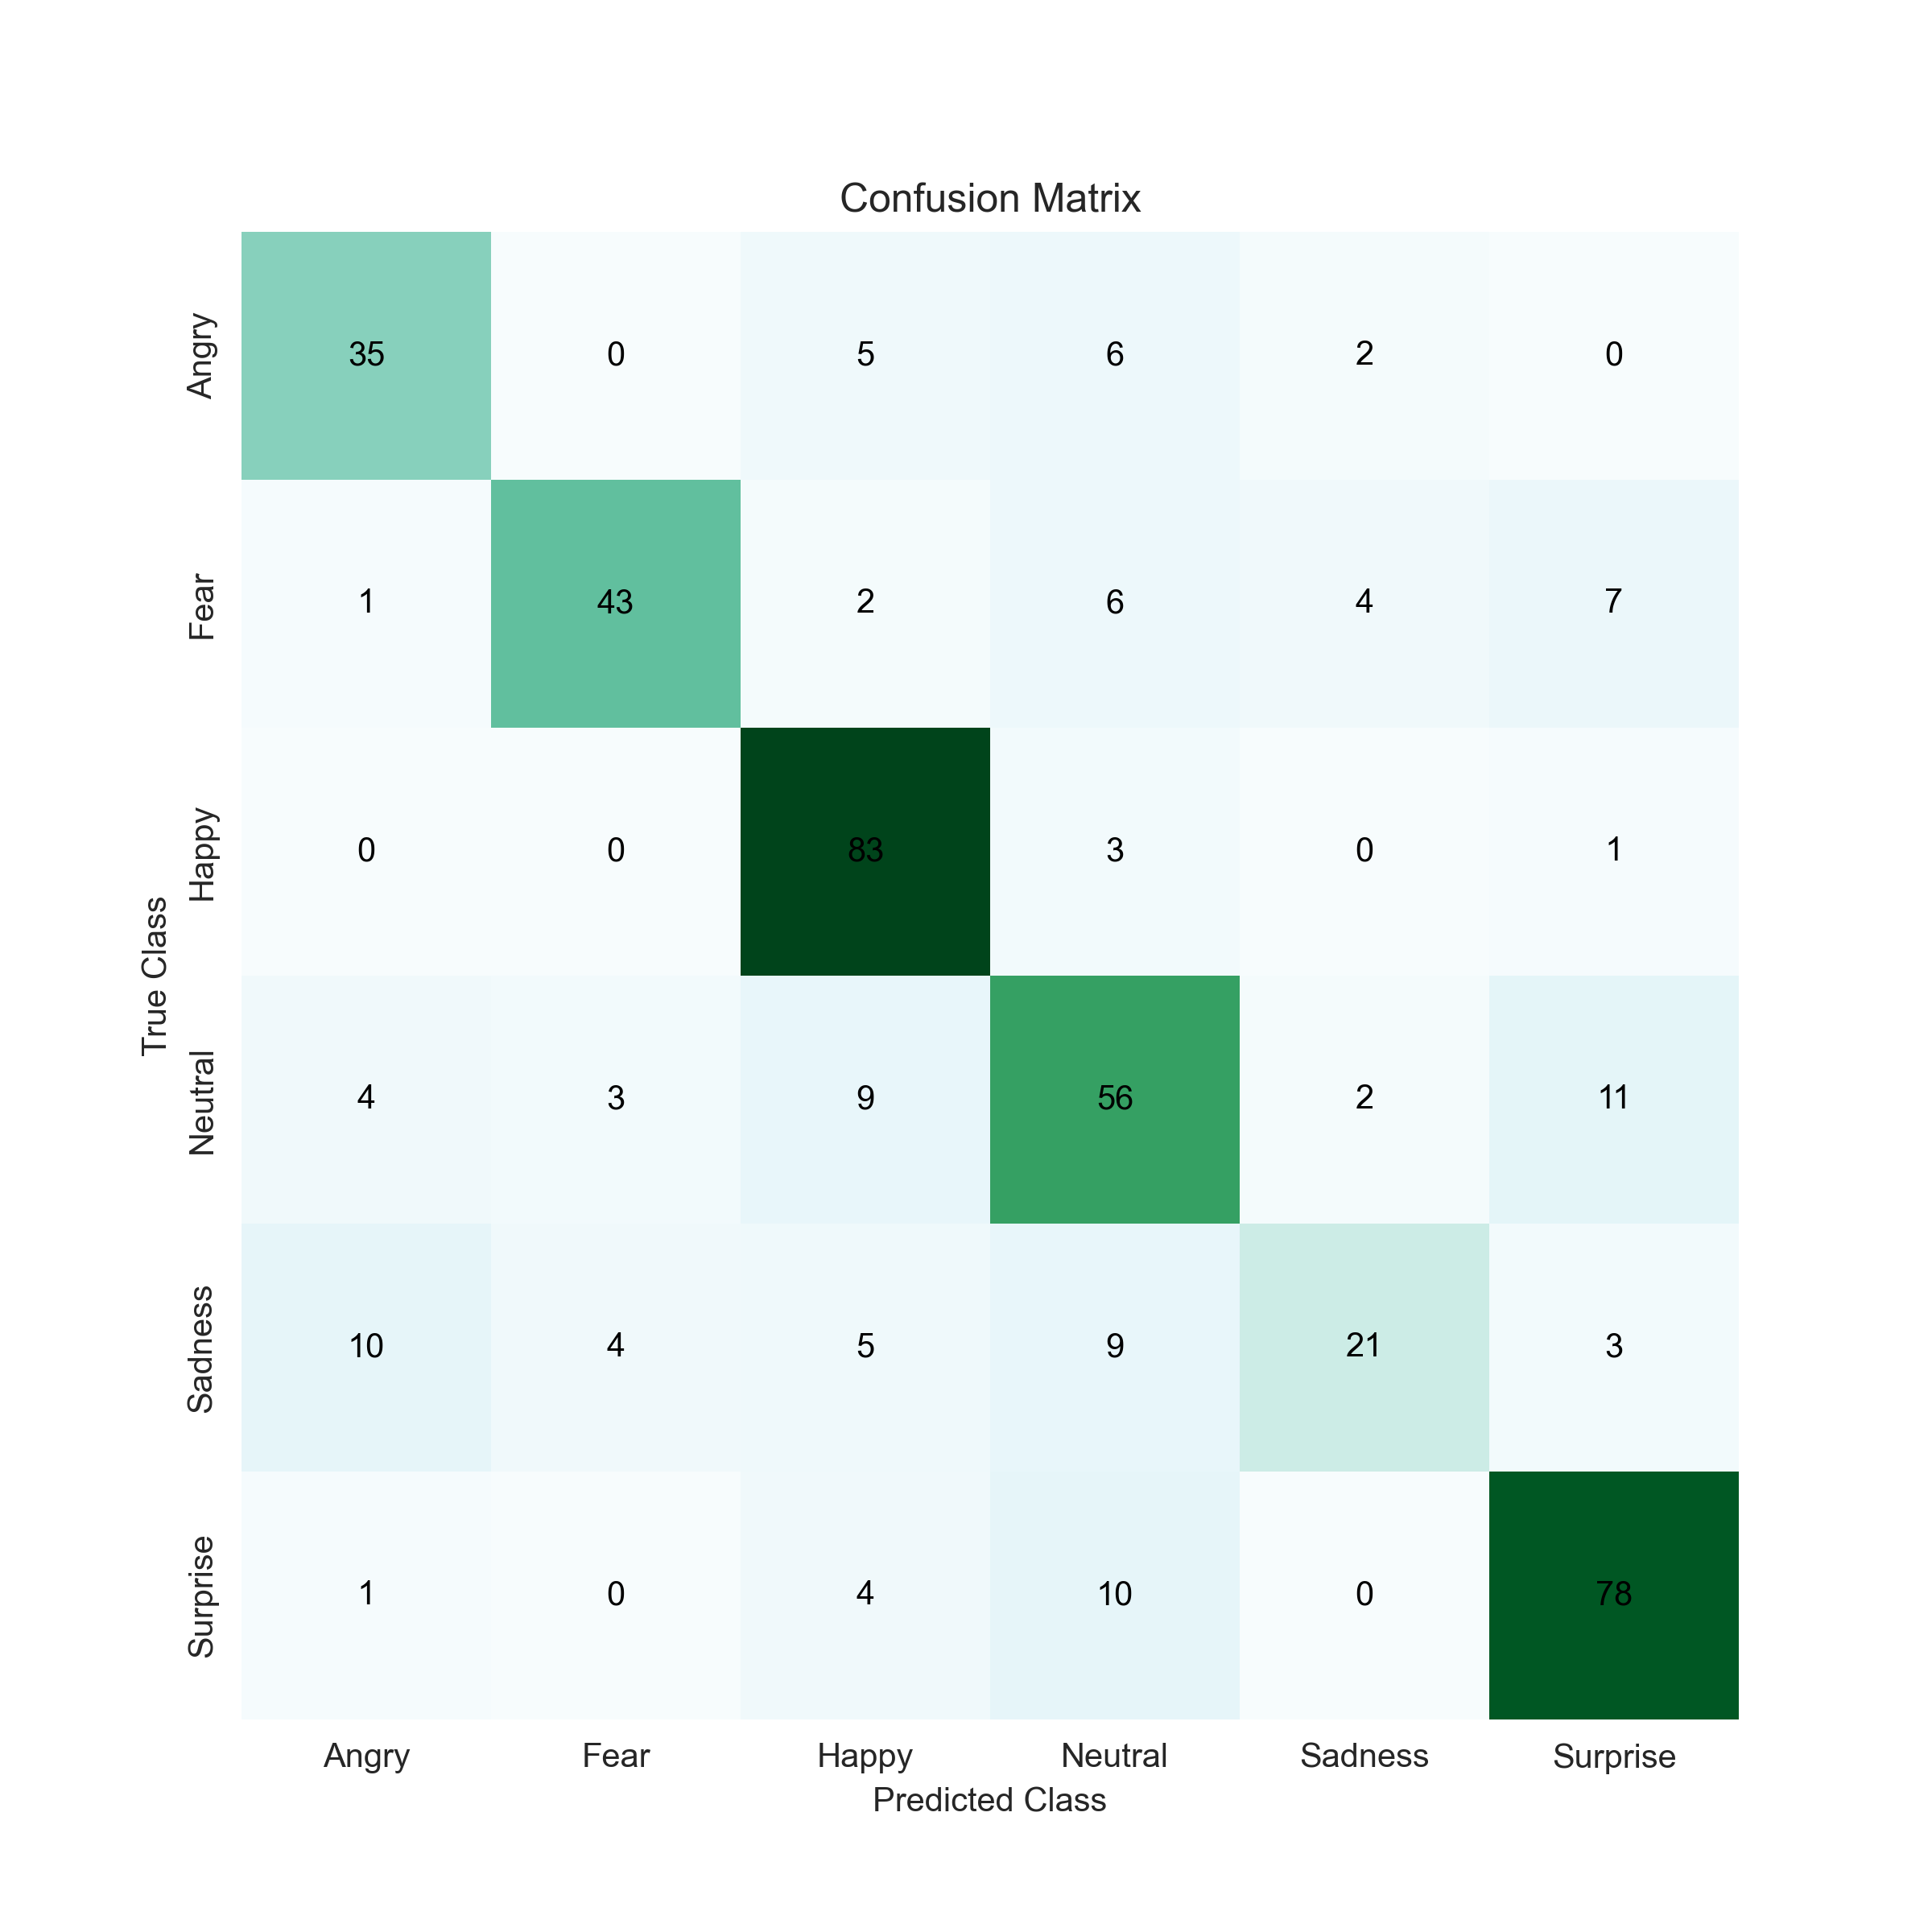
\includegraphics[width=1\textwidth]{figures/ConfusionMatrix_SVM.png}
	\caption{SVM - True Emotion vs. Predicted Emotion}
	\label{fig:confusionMatrix}
\end{figure}

\begin{figure}[h]
	\centering
	\includegraphics[width=1\textwidth]{figures/FeatureExtractionComparison.png}
	\caption{Feature Extraction Comparison: LBP vs. HOG}
	\label{fig:featureExtraction}
\end{figure}

\begin{figure}[h]
	\centering
	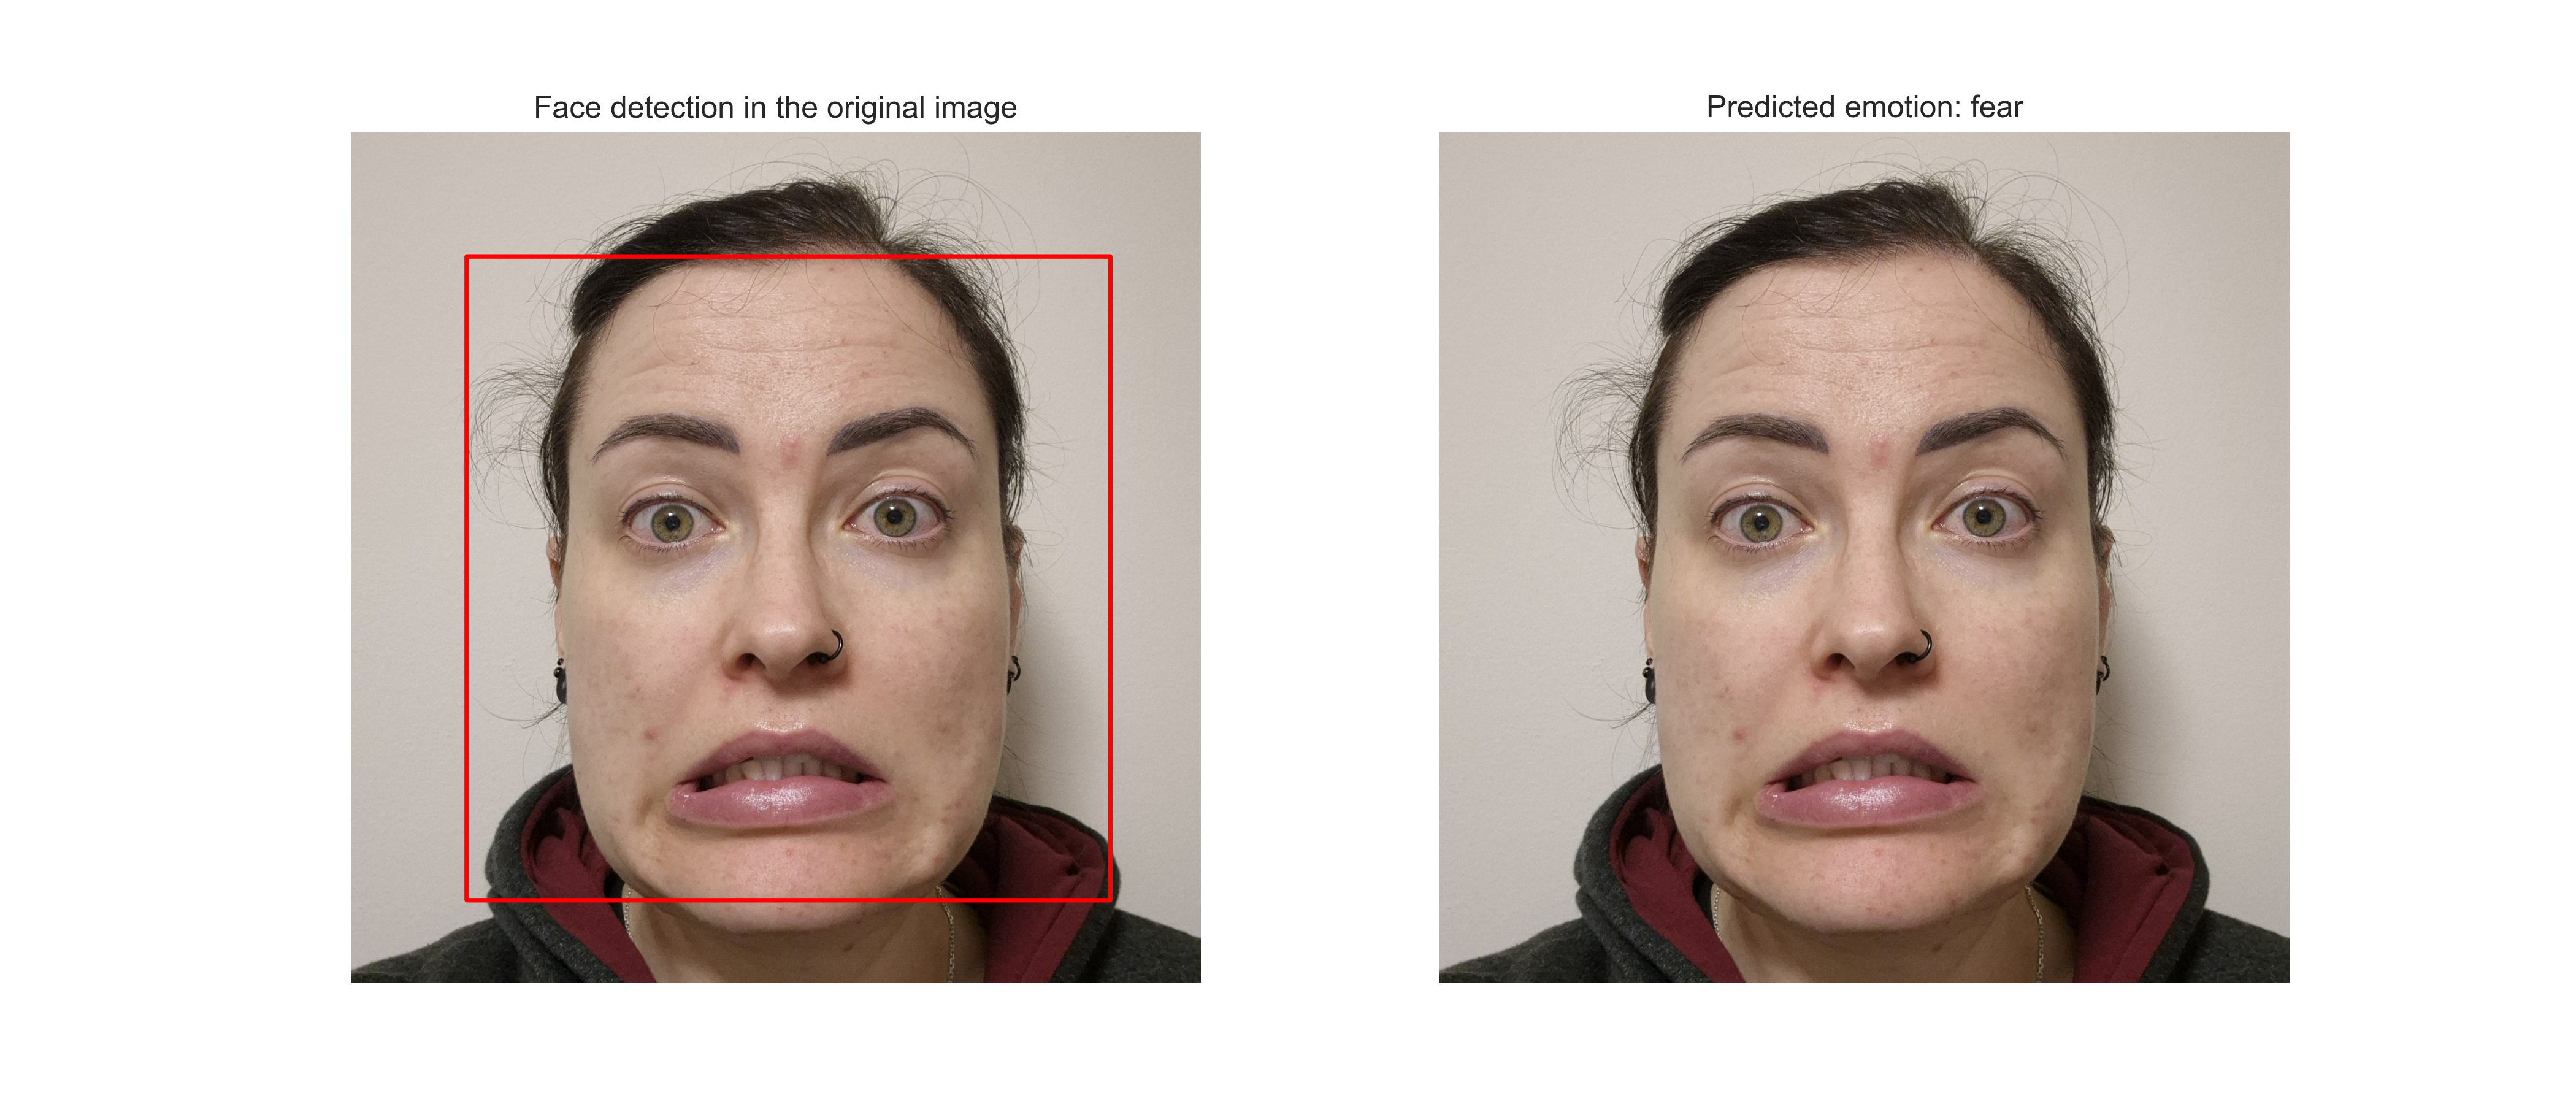
\includegraphics[width=1\textwidth]{figures/DetectionAndPrediction_fear.png}
	\caption{Correctly predicted emotion - fear}
	\label{fig:predictionFear}
\end{figure}

\begin{figure}[h]
	\centering
	\includegraphics[width=1\textwidth]{figures/DetectionAndPrediction_happy.png}
	\caption{Correctly predicted emotion - happy}
	\label{fig:predictionHappy}
\end{figure}

\begin{figure}[h]
	\centering
	\includegraphics[width=1\textwidth]{figures/DetectionAndPrediction_neutral.png}
	\caption{Correctly predicted emotion - neutral}
	\label{fig:predictionNeutral}
\end{figure}

\begin{figure}[h]
	\centering
	\includegraphics[width=1\textwidth]{figures/DetectionAndPrediction_surprise.png}
	\caption{Correctly predicted emotion - surprise}
	\label{fig:predictionSurprise}
\end{figure}

\begin{figure}[h]
	\centering
	\includegraphics[width=1\textwidth]{figures/DetectionAndPrediction_anger.png}
	\caption{Wrongly predicted emotion - True emotion: sadness}
	\label{fig:predictedAnger}
\end{figure}

\begin{figure}[h]
	\centering
	\includegraphics[width=1\textwidth]{figures/DetectionAndPrediction_sadness.png}
	\caption{Wrongly predicted emotion - True emotion: anger}
	\label{fig:predictionSad}
\end{figure}
